% !TeX root = ../main.tex
% Add the above to each chapter to make compiling the PDF easier in some editors.

\chapter{Results and Analysis}\label{chapter:results and analysis}

\section{Model Performance Analysis}

\subsection{Comparison with benchmark models}

\begin{itemize}
    \item ARIMA model
    \item Markets are efficient, and all investors have access to the same information.
    \item Asset returns are normally distributed and can be described by their mean (expected return) and variance (risk).
\end{itemize}

\paragraph{Comparison with ARIMA}

MSE, Present the prediction accuracy of the GPR models for the target assets.


\subsection{Analysis of prediction intervals}

\subsection{Model robustness and generalization}

\section{Portfolio Optimization Outcomes}


\subsection{Strategy Performance Comparison}
Return analysis
\begin{figure}[h]
    \centering
    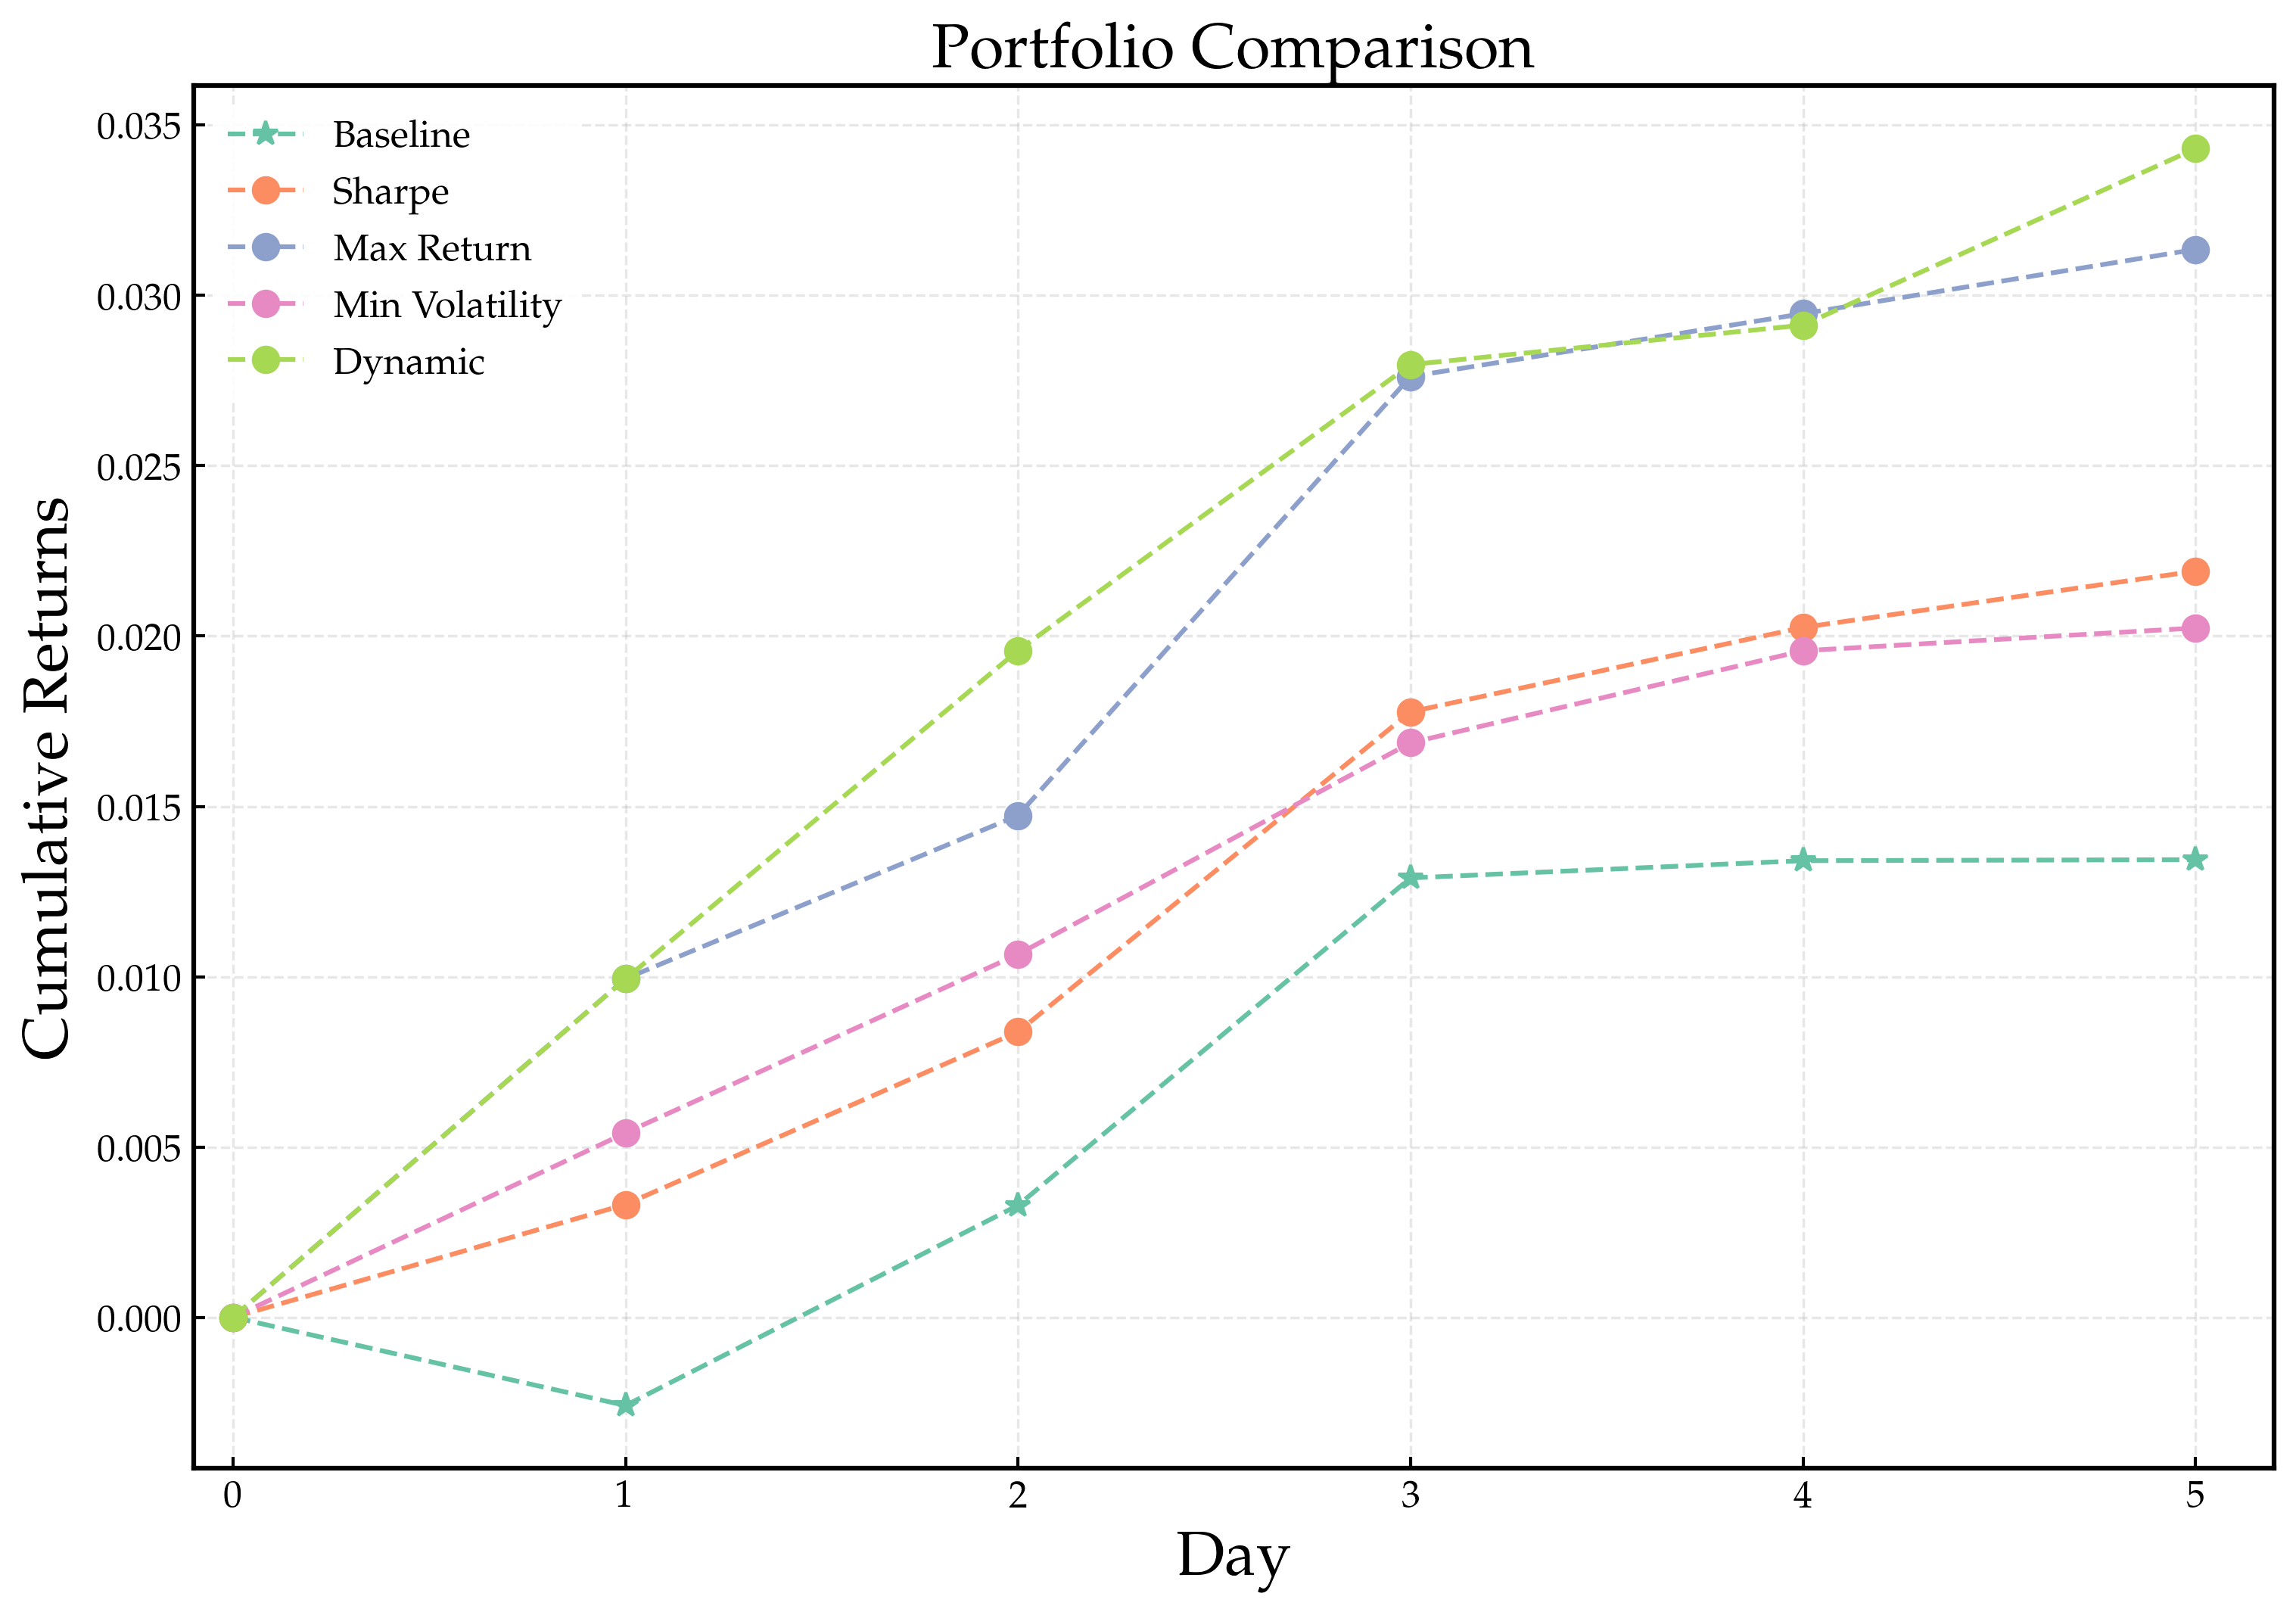
\includegraphics[width=0.6\textwidth]{figures/portfolio_comparison.png}
    \caption{Portfolio Comparison}
    \label{fig:portfolio_comparison}
\end{figure}

Risk metrics
Transaction costs impact

\begin{figure}[h]
    \centering
    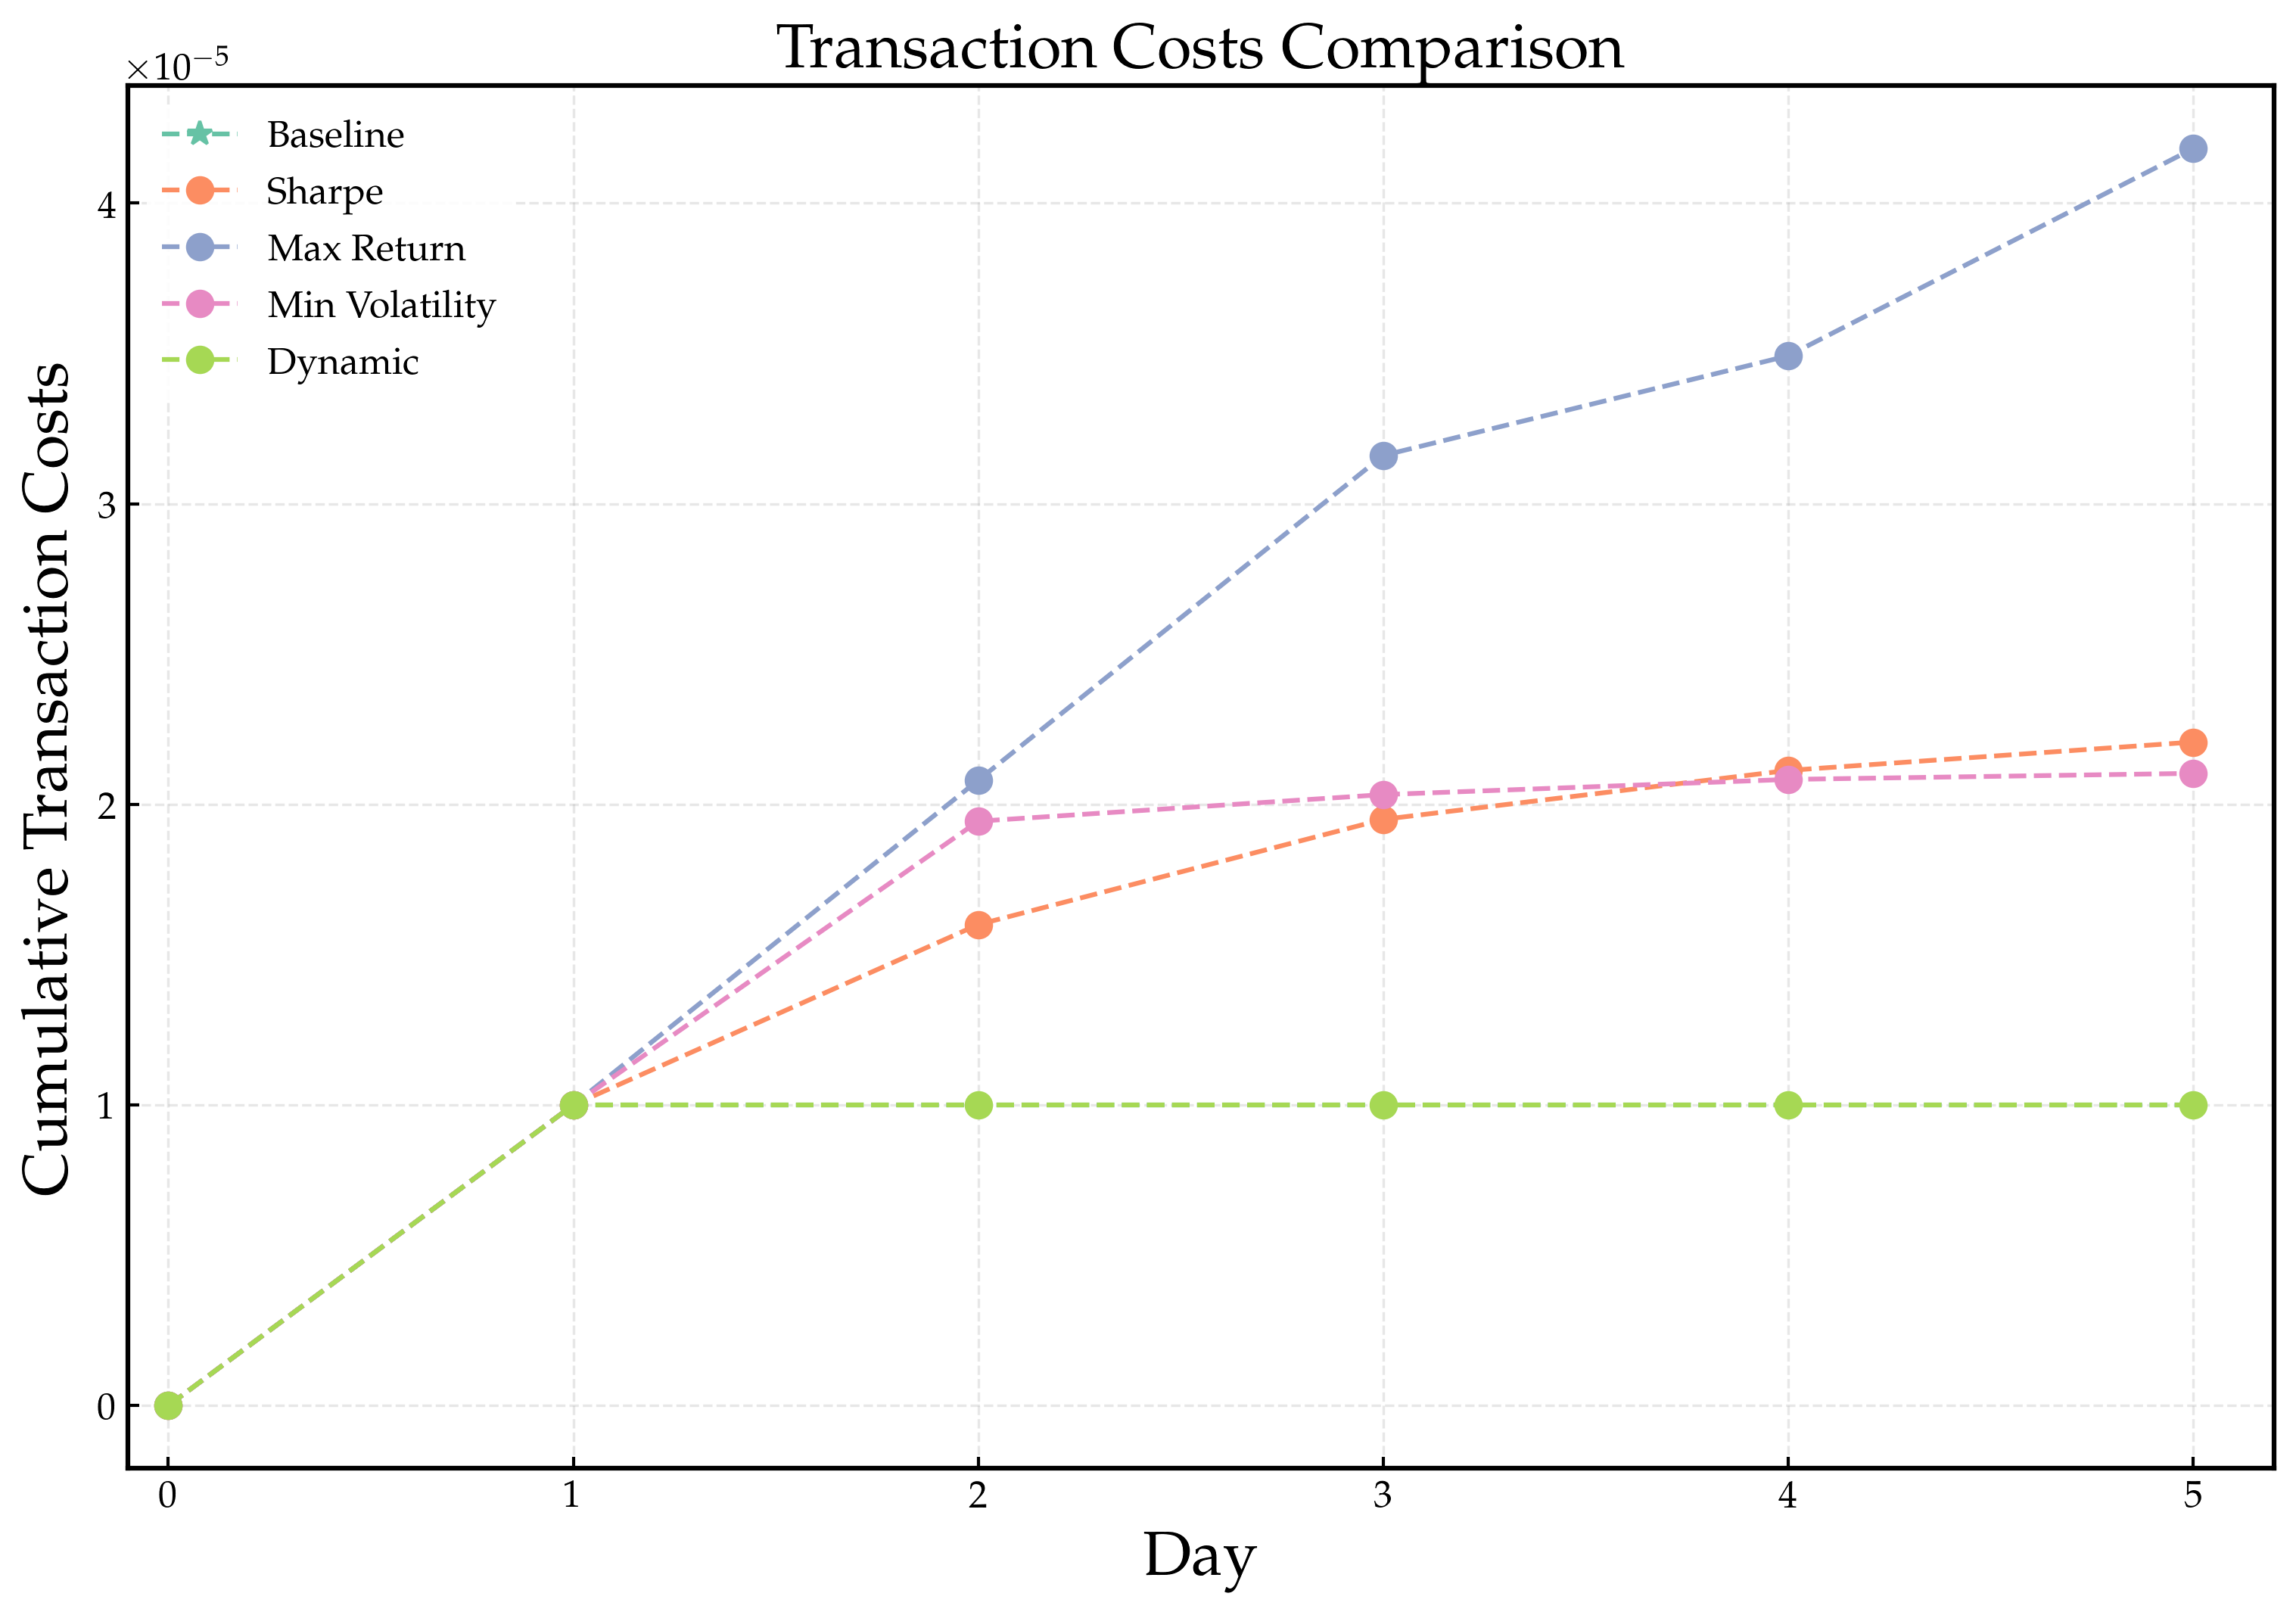
\includegraphics[width=0.6\textwidth]{figures/trx_costs_comparison.png}
    \caption{Transaction Costs Comparison}
    \label{fig:trx_costs_comparison}
\end{figure}

Strategy switching frequency analysis


Comparative Analysis:
Compare the performance of all strategies, highlighting the strengths and weaknesses of each.

\subsection{Dynamic Strategy Evaluation}
Probability threshold sensitivity
Strategy switching effectiveness
Portfolio turnover analysis
Risk-adjusted performance metrics

\section{Backtesting Results}
Provide detailed results from the backtesting, including cumulative returns, volatility, Sharpe ratios, and transaction costs for each strategy.

\subsection{Transaction Costs impact}


\section{Robustness Tests}

\subsection{Different market conditions}

\subsection{Hyperparameter sensitivity}

\subsection{Out-of-sample performance}

\subsection{Statistical significance tests}


